
\FloatBarrier
\section{Колебательная система с гистерезисом в возвращающей силе} %  % {{{1 _VGLASS_
\label{atu:sect:vglass}

\LinkRef{
  vglass: ITMM-2013
}

\subsection{Определение системы и анализ её динамики} %  % {{{2 _vglass_task

Колебательные системы с различными видами нелинейностями
как в возвращающей силе, так и члене при первой производной,
часто рассматриваются как потенциальные кандидаты в хаотические системы.
Особый интерес представляют системы, нелинейные компоненты которых
отображают реальные элементы систем управления~\cite{atu_st85,atu_ISDMCI2013,atu_asau20}.
Одним из таких существенно нелинейных элементов
является гистерезис. % TODO: cite
Рассмотрим изначально неустойчивую  систему,
которая стабилизируется релейно-пропорциональным
стабилизирующим воздействием.
Такая система стабилизации активируется при заданном отклонении наблюдаемой
величины, а выключается при меньшем. Такая неоднозначность в поведении
систем стабилизации приводит к разнообразным колебательным явлениям вблизи
точки стабилизации, а все попытки линеаризации рассматриваемых
нелинейностей, в данном случае, приводят к принципиальным ошибкам в
моделировании.

Наличие точки неустойчивого равновесия, требующего стабилизирующего
воздействия в большем масштабе, явной, а зачастую и скрытой нелинейности
элементов системы, априорная параметрическая неопределенность внешних
воздействий, --- всё это создаёт предпосылки для появления у систем сложной
колебательной динамики, в том числе и хаотической.
Рассмотрим уравнение, задающее динамику этой системы:
%
\begin{equation}
  \ddot{x} + c_o \dot{x} + r( x, \ldots ) = u(t),
  \label{atu:eq:vglass}
\end{equation}
%
где
$x(t)$ -- координата (выходной сигнал),
$ c_0$ -- безразмерный коэффициент демпфирования,
$u(t) = U_{in} \sin( \omega_{in} t ) $ -- внешняя возмущающая сила,
$r( x, \ldots) $ --- возвращающая сила,
включающая линейную составляющую ($ax$, $a<0$),
обуславливающую неустойчивость при малых отклонениях,
и гистерезисную компоненту, которая задаётся алгоритмически.
Характерный вид возвращающий силы приведён на  рис.~\ref{atu:f:vg_rf}.

\begin{figure}[htb!]
\centerline{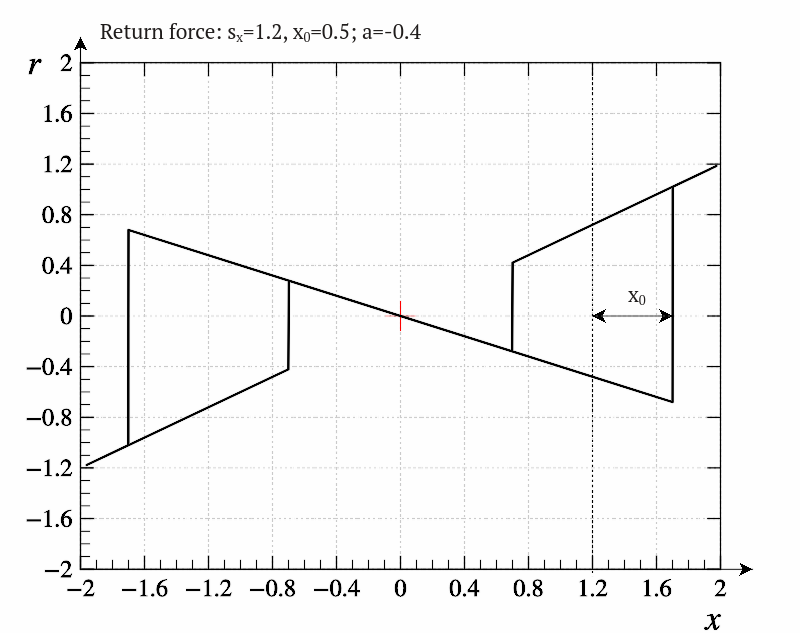
\includegraphics[width=0.5\textwidth]{p/cha/vg/vg_rf-p_rf.png} }
\caption{Гистерезисная возвращающая сила}
\label{atu:f:vg_rf}
\end{figure}

Параметрами этой зависимости, помимо уже упомянутого коэффициента $a$,
являются $s_x$ --- центральная точка включения и выключения
стабилизирующего воздействия,
$x_0$ --- полуширина гистерезиса.
Ширина петли гистерезиса для данной системы определяет
энергию, которую получает система от системы стабилизации в процессе работы.
Именно это величина и будет идентифицируемым параметром.


В отличие от системы Дуффинга, рассматриваемая система имеет собственную
динамику при отсутствии возмущающего воздействия.
При малых значениях $x_0$ происходят нелинейные,
но достаточно простые колебания по одну сторону от
точки $x=0$~(рис.~\ref{atu:f:vglass_phase_f_u00}),
причём сторона определяется начальными условиями.
Спектр колебаний весьма бедный.

\begin{figure}[ht!]
\begin{center}
  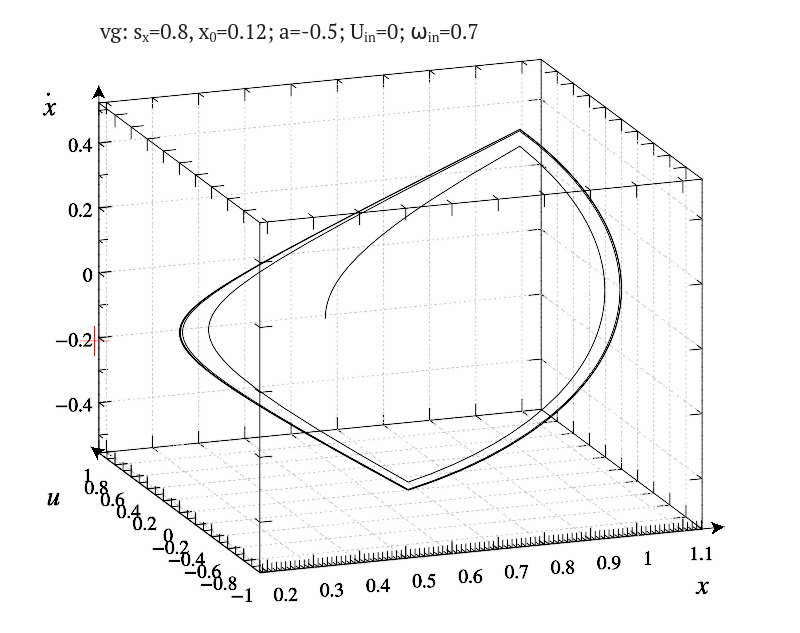
\includegraphics[width=0.49\textwidth]{p/cha/vg/vg_0-p_phe_0x00_0x70_0x12.png}
  \hfill
  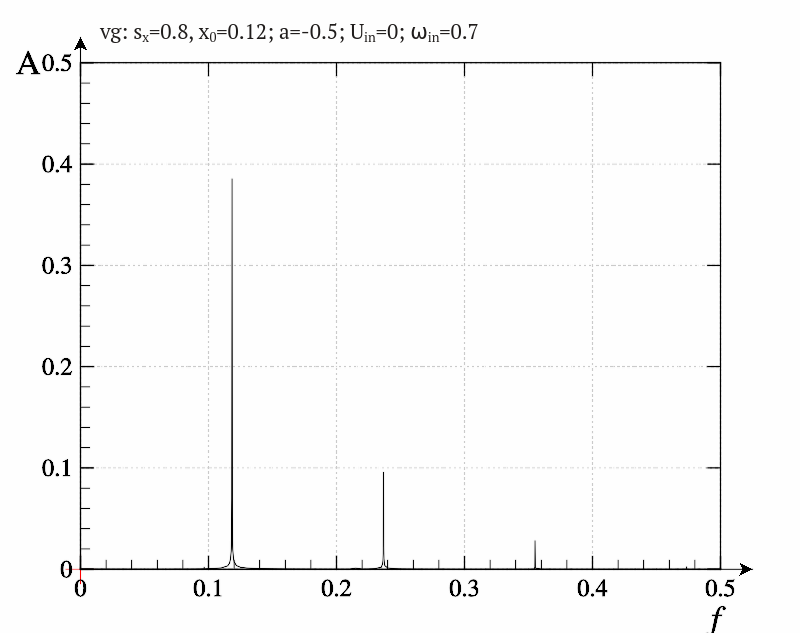
\includegraphics[width=0.49\textwidth]{p/cha/vg/vg_fft-p_f_0x00_0x70_0x12.png}
\end{center}
  \caption{Расширенный фазовый портрет и спектр системы (\ref{atu:eq:vglass}) при $U_{in}=0$ и $x_0=0.12$}
\label{atu:f:vglass_phase_f_u00}
\end{figure}

При росте параметра $x_0$ динамика системы становится более сложной
(рис.~\ref{atu:f:vglass_phase_f_u01}),
однако спектр системы остаётся простым линейчатым.
Такое поведение сохраняется вплоть до естественного ограничения $x_o < s_x$,
при этом фазовый портрет приближается к окружности.

\begin{figure}[ht!]
\begin{center}
  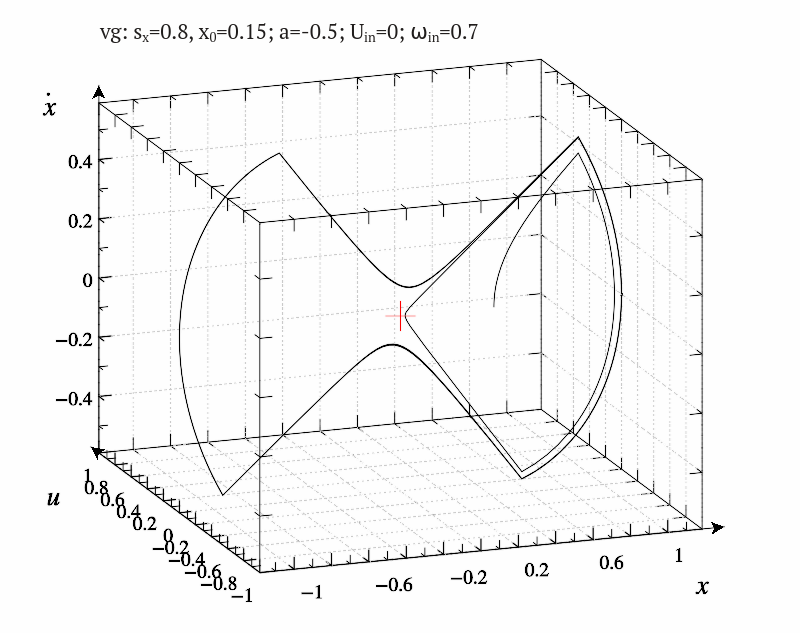
\includegraphics[width=0.49\textwidth]{p/cha/vg/vg_0-p_phe_0x00_0x70_0x15.png}
  \hfill
  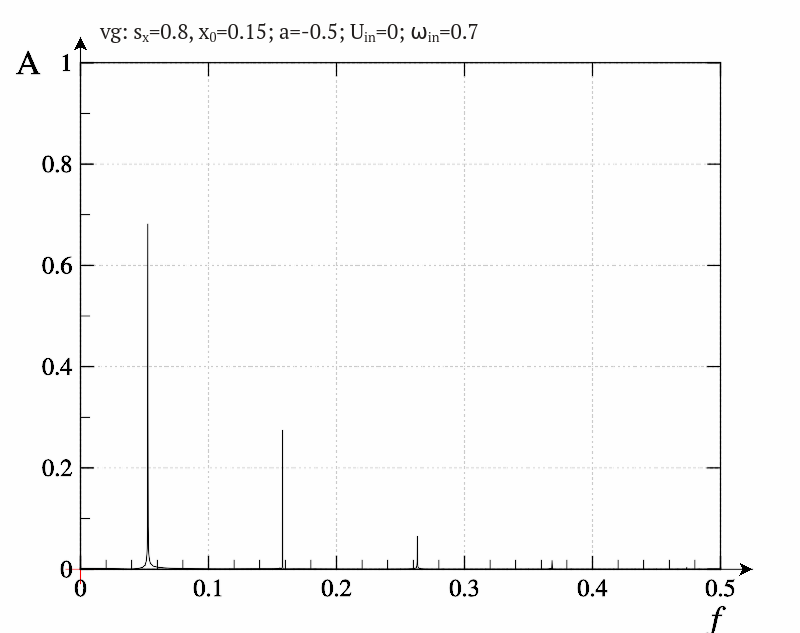
\includegraphics[width=0.49\textwidth]{p/cha/vg/vg_fft-p_f_0x00_0x70_0x15.png}
\end{center}
  \caption{Расширенный фазовый портрет и спектр системы (\ref{atu:eq:vglass}) при $U_{in}=0$ и $x_0=0.15$}
\label{atu:f:vglass_phase_f_u01}
\end{figure}

При наличии ненулевого внешнего воздействия $u(t)$
картина заметно усложняется.
Наблюдаются такие значения параметра $x_0$,
при которых наблюдается сложный аттрактор, характерный для
хаотической динамики~(рис.~\ref{atu:f:vglass_phase_f_u10})
и участки сплошного спектра.

\begin{figure}[ht!]
\begin{center}
  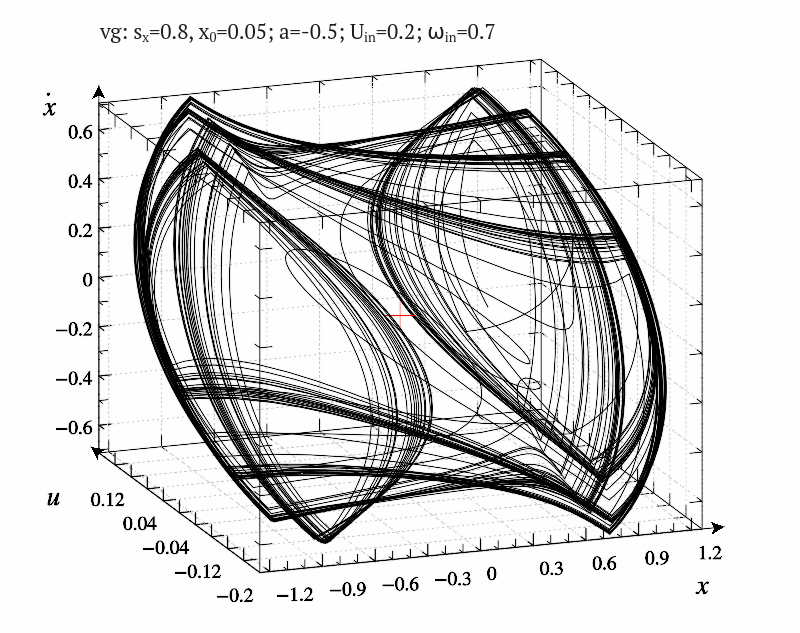
\includegraphics[width=0.49\textwidth]{p/cha/vg/vg_0-p_phe_0x20_0x70_0x05.png}
  \hfill
  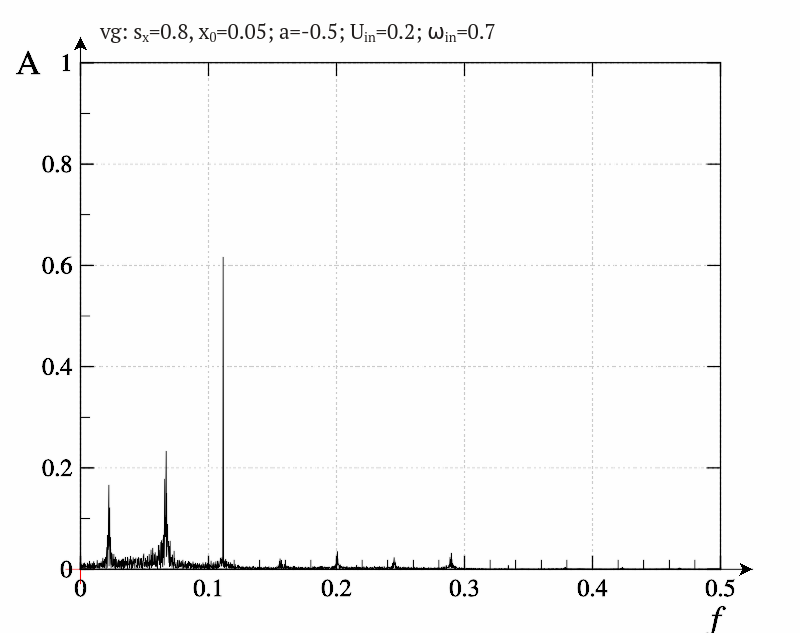
\includegraphics[width=0.49\textwidth]{p/cha/vg/vg_fft-p_f_0x20_0x70_0x05.png}
\end{center}
  \caption{Расширенный фазовый портрет и спектр системы (\ref{atu:eq:vglass}) при $U_{in}=0.2$ и $x_0=0.05$}
\label{atu:f:vglass_phase_f_u10}
\end{figure}

Общим свойством этой системы и системы Дуффинга является то,
что участок сплошного спектра примыкает к точке нулевой частоты,
что затрудняет процесс усреднения критерия.

Также наблюдаются такие диапазоны $x_0$,
в которых наблюдаются регулярные колебания
(рис.~\ref{atu:f:vglass_phase_f_u11}).

\begin{figure}[ht!]
\begin{center}
  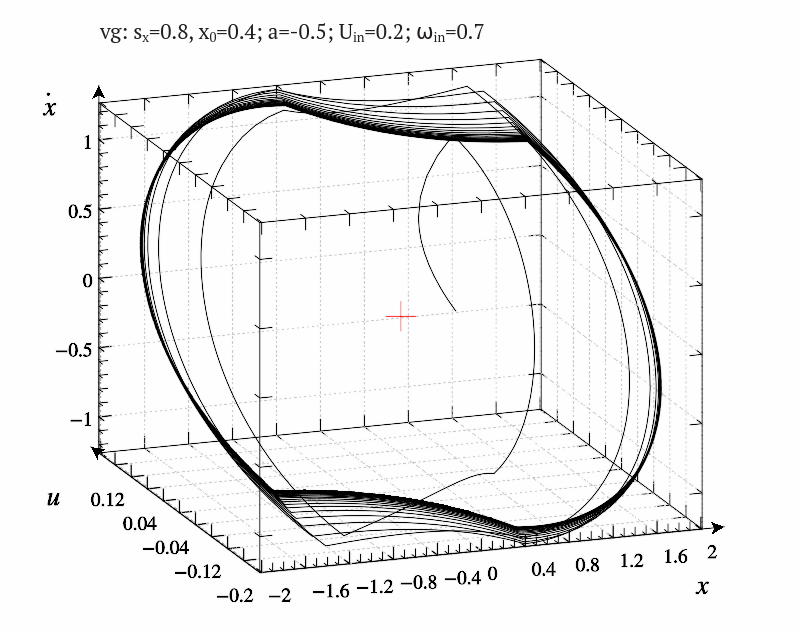
\includegraphics[width=0.49\textwidth]{p/cha/vg/vg_0-p_phe_0x20_0x70_0x40.png}
  \hfill
  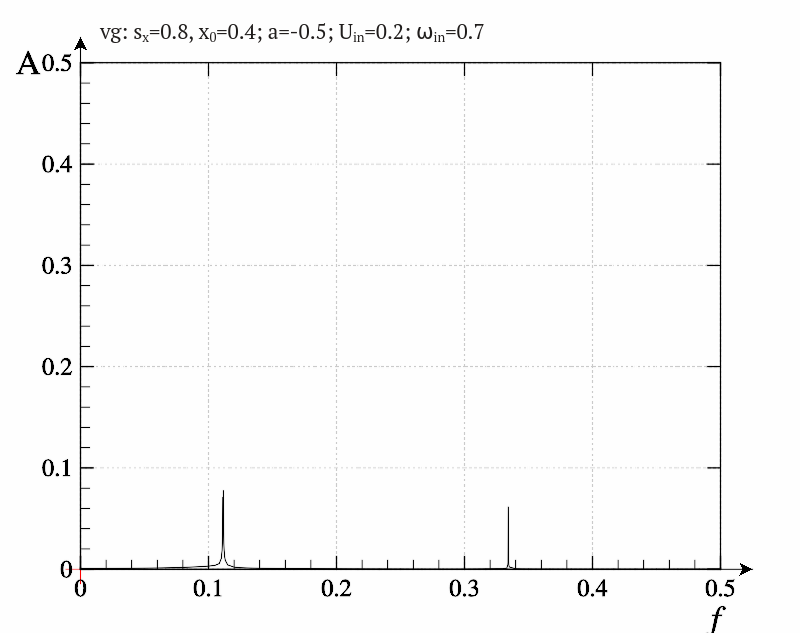
\includegraphics[width=0.49\textwidth]{p/cha/vg/vg_fft-p_f_0x20_0x70_0x40.png}
\end{center}
  \caption{Расширенный фазовый портрет и спектр системы (\ref{atu:eq:vglass}) при $U_{in}=0.2$ и $x_0=0.40$}
\label{atu:f:vglass_phase_f_u11}
\end{figure}

Помимо регулярных колебаний, наблюдаются
режимы сложно-периодической динамики,
с сложным аттрактором и спектром,
в котором наблюдаются ряд близко расположенных пиков
(рис.~\ref{atu:f:vglass_phase_f_u12}).

\begin{figure}[ht!]
\begin{center}
  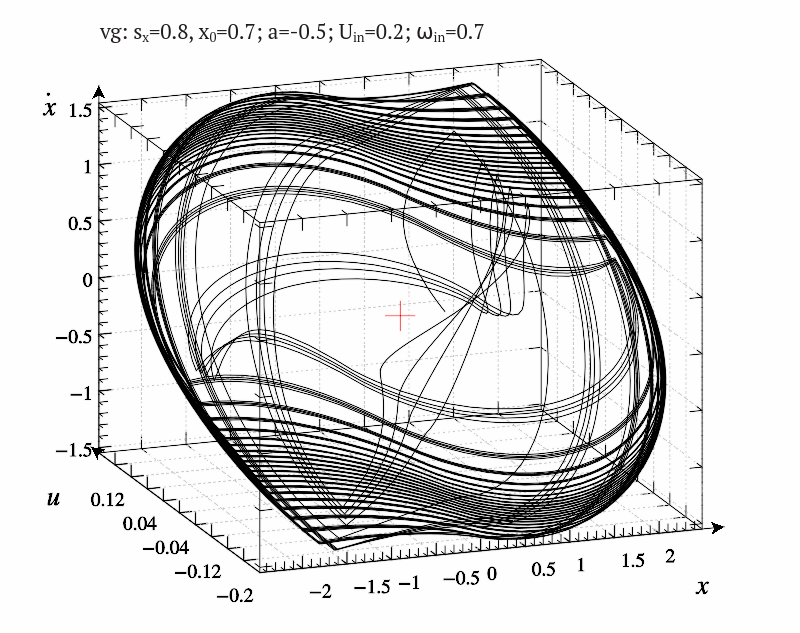
\includegraphics[width=0.49\textwidth]{p/cha/vg/vg_0-p_phe_0x20_0x70_0x70.png}
  \hfill
  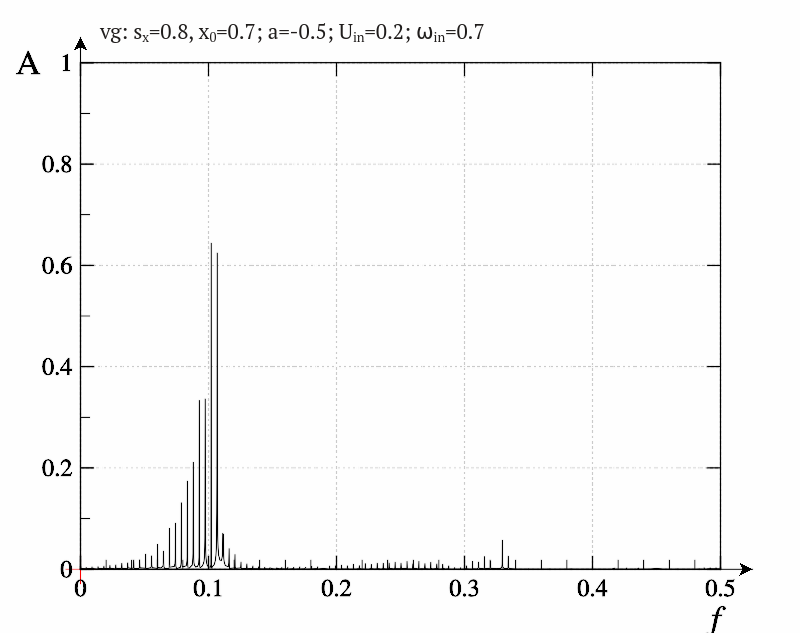
\includegraphics[width=0.49\textwidth]{p/cha/vg/vg_fft-p_f_0x20_0x70_0x70.png}
\end{center}
  \caption{Расширенный фазовый портрет и спектр системы (\ref{atu:eq:vglass}) при $U_{in}=0.2$ и $x_0=0.70$}
\label{atu:f:vglass_phase_f_u12}
\end{figure}

Такое поведение сложно, а в случае нестационарного значения параметра
может быть и невозможно отличить от хаотического поведения.

Таким образом, так как система в рабочем диапазоне параметра
$x_0$ демонстрирует различные виды динамик, в том числе хаотическую,
то для идентификации имеет смысл рассмотреть набор методов,
рассматриваемых в данной работе.


\subsection{Анализ и выбор критерия}  % {{{2

При синтезе критерия для нелинейной колебательной системы,
если нет возможности использовать
какой-либо явный и очевидный критерий,
в первую очередь следует рассмотреть
критерии вида $q_{x^2}$, $q_{rx}$ и $q_T$.
Так как гистерезисная возвращающая сила
не даёт возможности использовать аналитический
подход, то рассмотрим
зависимости $q_{rx}$ и $q_T$
(рис.~\ref{atu:f:vglass_q}),
полученные путём численного моделирования.

\begin{figure}[ht!]
\begin{center}
  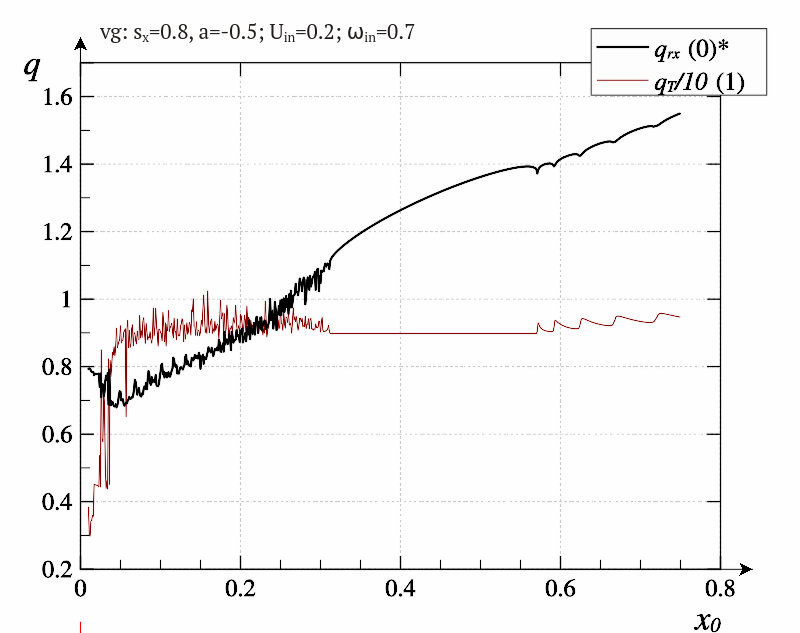
\includegraphics[width=0.49\textwidth]{p/cha/vg/vg_q1-p_q.png}
\end{center}
  \caption{Зависимости $q_{rx}(x_0)$ и $q_T(x_0)$ для системы (\ref{atu:eq:vglass})}
\label{atu:f:vglass_q}
\end{figure}

Анализ зависимостей позволяет сделать вывод о том, что критерий $q_T$
не пригоден для идентификации параметра $x_0$
рассматриваемой системы, ввиду того,
что зависимости от параметра, если не принимать во внимание колебания,
практически отсутствует.

Применений критерия $q_{rx}$ достаточно противоречиво.
С одной стороны, в целом наблюдается близкая к линейной зависимость,
что снижает требования к тонкой настройке системы идентификации.
С другой стороны, на тех участках,
где наблюдаются переходы от сложно-периодических колебаний
к хаотическим, монотонность зависимости нарушается.
Однако, амплитуда этих возмущений невелика,
что даёт возможность построения работоспособной системы идентификации,
но с существенными ограничениями на достижимую точность.
Таким образом, на неимением лучшего, будем использовать этот критерий.



% }}}2

\subsection{Тестовая задача идентификации}  % {{{2

% }}}2

\subsection{Влияние параметров системы идентификации на ошибку идентификации}  % {{{2

% }}}2


\subsection{Выводы}  % {{{2

Результаты моделирования
как динамики системы~(\ref{atu:eq:vglass})
так и процессов идентификации её параметра $x_0$
позволяют в сделать следующие выводы:

% }}}2

% }}}1

% vim: fdm=marker ft=tex
